%!TEX root = proyecto.tex

\chapter{Diseño y resolución}

%\linespread{1.5}

\section{Paul Viola and Michael Jones} \label{haar-like}

En 2001, el reconocimiento facial tuvo su primera aparición en el campo de la visión artificial como aplicación en tiempo real. Este avance fue de la mano de Paul Viola y Michael Jones. Análogamente, el punto de partida del estudio de este TFG. Durante este apartado, se estudiará el funcionamiento del algoritmo \textit{Viola-Jones face detector}, ideado por estos dos investigadores y se realizará una implementación del mismo mediante \textit{Python} y \textit{OpenCV} para comprobar como se comporta en la situación actual.

\subsection*{Método de estudio}

El trabajo de los expertos fue presentado por parte de la Universidad de Cambridge mediante un \textit{paper} (ensayo de la investigación). Y se introduce como: 
\begin{quote}
	"This paper describes a machine learning approach for visual object detection which is capable of processing images extremely rapidly and achieving high detection rates" \cite{paulViola}
\end{quote}

Para poder lograr esta afirmación se basan en un procedimiento de trabajo en dos fases: entrenamiento y detección. Igualmente, Paul y Michael dividen el proyecto en tres ideas principales para poder lograr un detector que se pueda ejecutar en tiempo real. Y estas son: la imagen integral, Adaboost (algoritmo de Machine Learning) y un método llamado \textit{attentional cascade structure}. 

Con todos estos puntos combinados lograron ingeniar un prototipo capaz de detectar caras humanas con un \textit{frame rate} de 15 fps. Fue diseñado para la detección de caras frontales, haciéndose difícil para posiciones laterales o inclinadas.

Las imágenes que se toman para realizar la detección pasan por una transformación del espacio de color a \textit{grayscale}. Con el objeto de encontrar características en ellas, llamadas \textit{haar-like features}. Nombradas así por su inventor Alfred Haar en el siglo XIX. En este trabajo se hacen uso de tres tipos de haar-like features, que son las siguientes:

\begin{figure}[htp]
	\centering
	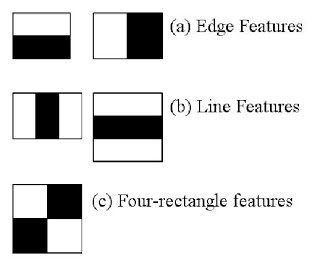
\includegraphics[width=5cm]{imagenes/haar-like.jpeg}
	\caption{Haar-like Features}
	\label{fig:haarLike}
\end{figure}

Las \textbf{\textit{Haar-like features}}, o también conocidas como \textit{Haar-wavelet} son una secuencia de funciones \textit{rescaled square-shaped}, siendo similares a las funciones de Fourier y con un comportamiento parecido a los \textit{Kernel} usados en las \textit{Redes Convolucionales} (matrices que consiguen extraer ciertas \textit{features} de la imagen de entrada). De manera que, las \textit{Haar Features} serán las características de la detección facial.

En un estudio ideal, los píxeles que forma el \textit{feature} tendrá una división clara entre píxeles de color blanco con los de color negro (Figura 4.1), pero en la realidad eso casi nunca se va a dar.

Más especificamente, las \textit{Haar-like features} están compuestas por valores escalares que representan la media de intensidades entre dos regiones rectangulares de la imagen. Estas capturan la intensidad del gradiente, la frecuencia espacial y las direcciones, mediante el cambio del tamaño, posición y forma de las regiones rectangulares basándose en la resolución que se define en el detector. \cite{haar-like}

Estas características van a ayudar al ordenador a entender lo que es la imagen estudiada. Van a ser utilizadas mediante \textit{Machine Learning} para detectar donde hay una cara o no, mediante un recorrido sobre toda la imagen. Esto conlleva una potencia de computación elevada. Para paliar este problema idearon el método de la \textit{Imagen Integral}.

La \textbf{\textit{Imagen Integral}} permite calcular sumatorios sobre subregiones de la imagen, de una forma casi instantánea. Además de ser muy útiles para las \textit{HAAR-like features}, también lo son en muchas otras aplicaciones.

Si se supone una imagen con unas dimensiones de $<w,h>$ (ancho y alto, respectivamente), la imagen integral que la representa tendrá unas dimensiones de $<w+1,h+1>$. La primera fila y columna de esta son ceros, mientras que el resto tendrán el valor de la suma de todos los píxeles que le preceden. \cite{integral-web} Ahora, para calcular la suma de los píxeles en una región especifica de la imagen, se toma la correspondiente en la imagen integral y se suma según la siguiente fórmula (siguiendo la numeración de la Figura \ref{fig:integral}):
\begin{center}
	$sum = L4 + L1 - (L2 + L3)$ 
\end{center}
\begin{figure}[htp]
	\centering
	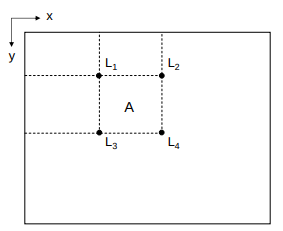
\includegraphics[width=5cm]{imagenes/integral.png}
	\caption{Funcionamiento de una \textit{Imagen Integral}}
	\label{fig:integral}
\end{figure}

Viola y Jones junta esta propuesta con los filtros \textit{Haar-like features}, y consiguen computar dichas características de manera constante y eficaz. \cite{integral}\\

% ---------------------------
%https://aishack.in/tutorials/integral-images-opencv/

%https://www.quora.com/How-integral-image-is-used-in-image-processing-and-how-improves-the-computation-time?share=1
%https://www.quora.com/What-are-the-must-read-papers-in-the-field-of-computer-vision-for-a-student-in-pursuing-research-in-the-field
% ---------------------------
%
% MACHINE LEARNING - ADABOOST
\newpage
Una vez estudiada la obtención de características y con un set de entrenamiento, solo queda seleccionar un método de \textit{machine learning} que permita crear una función de clasificación. Concretamente, se plantea el uso de una variante de \textbf{\textit{AdaBoost}}, que permite seleccionar un pequeño conjunto de características y poder entrenar un clasificador. 

Este algoritmo de aprendizaje esta basado en generar una predicción muy buena a partir de la combinación de predicciones peores y más débiles, donde cada uno de estas se corresponde con el \textit{threshold} de una de las características \textit{Haar-like}. La primera vez que aparece este algoritmo, de forma práctica, fue de la mano de \textit{Freund y Schapire} \cite{adaboost1}. Sin embargo, el usado por \textit{Viola y Jones} es una modificación de este.

La salida que genera el algoritmo \textbf{\textit{AdaBoost}} es un clasificador llamado \textit{Strong Classifier}, como se ha mencionado anteriormente, compuesto por combinaciones lineales de \textit{Weak Classifiers}. 

El procedimiento para encontrar \textit{Weak Classifiers} es ejecutar el algoritmo T iteraciones donde T es el número de clasificadores a encontrar. En cada iteración, el algoritmo busca el porcentaje de error entre todas las características y escoge la que menos porcentaje de error presente en dicha iteración. (Como se muestra en la \textit{Figura \ref{fig:ada1}}) \cite{adaboost2}

\begin{figure}[htp]
	\centering
	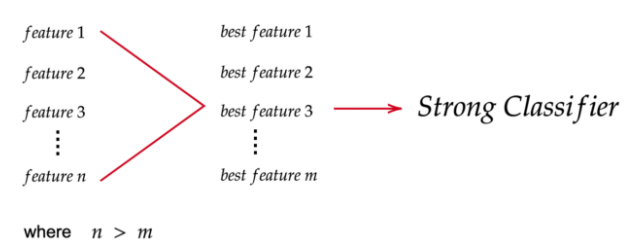
\includegraphics[width=10cm]{imagenes/ada1.png}
	\caption{Construcción del \textit{Strong Classifier}}
	\label{fig:ada1}
\end{figure}

Con estos clasificadores se procede a la construcción de una estructura en cascada para crear un \textit{Multi-stage Classifier}, que podrá realizar una detección rápida y buena. Por tanto, la estructura de cascada esta compuesta por varios estados de \textit{Strong Classifiers} generados por el algoritmo \textit{AdaBoost}. Donde el trabajo de cada estado será identificar si, dada una región de la imagen, no hay una cara o si hay la posibilidad de que la haya. \cite{adaboost1}

Si el resultado de uno de los estados es que no existe una cara en dicha región, esta se descarta directamente. Mientras que, si hay la posibilidad de que exista una, pasa al siguiente estado de la estructura. De tal forma que, cuantos más estados atraviese una región de la imagen, con más seguridad se podrá afirmar que existe una cara en ella. La estructura completa se refleja en la \textit{Figura \ref{fig:ada2}}.

\begin{figure}[htp]
	\centering
	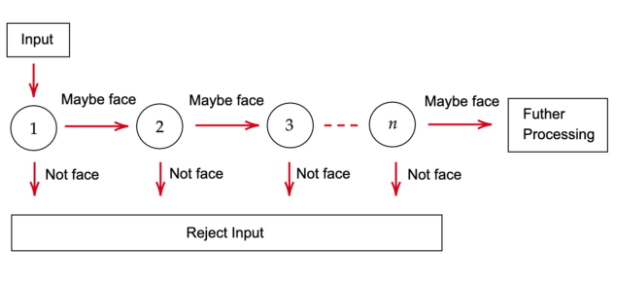
\includegraphics[width=10cm]{imagenes/ada2.png}
	\caption{Construcción del \textit{Multi-stage Classifier}}
	\label{fig:ada2}
\end{figure}

% VIDEO DE LOCOS: https://www.youtube.com/watch?v=uEJ71VlUmMQ&t=5s

\subsection*{Implementación y Experimentación}

El prototipo será implementado en \textit{Python}, con el uso de \textit{OpenCV}. Y, el objetivo es construir dos detectores de caras, donde el primero usará un modelo preentrenado de \textit{OpenCV} de caras frontales. Mientras que en el segundo, se intentará modificar el programa, para que mediante el uso de varios modelos preentrenados se pueda detectar una cara con una mascarilla.

La \textbf{implementación básica} hace uso de un modelo preentrenado cargado mediante una clase de \textit{OpenCV} llamada \textit{Cascade Classifier}. Esta representa la base de \textit{Machine Learning} explicado en el apartado anterior. Asimismo, \textit{OpenCV} también proporciona una serie de archivos \textit{xml} con diferente modelos preentrenados. En concreto, para este prototipo se hace uso del modelo por defecto, detector de caras frontal, como se muestra en la investigación de \textit{Viola y Jones}.

Finalmente, la detección se realiza, tras realizar una transformación del espacio de color a blanco y negro, mediante la función \textit{detectMultiScale} de la clase, creada anteriormente, \textit{Cascade Classifier}. Concretamente, su funcionalidad será encontrar caras dentro de las imágenes que vaya procesando.

[Explicacion del prototipo custom]

\textbf{OpenCV y Haar-like features + Machine Learning con PCA y SVM}
% Buscar como referencia para lo segundo HOG y SVM

Se implementa un identificador de caras conjunto a un modelo de \textit{Machine Learning} que identifica cuando una persona lleva o no mascarilla, mediante una toma de muestras anterior. Gracias a los modelos PCA y SVM, se puede crear un modelo para su identificador.
Lo malo: Solo funciona con los rostros/rostro que se toma como referencia para construir el modelo, igualmente pasa con el tipo de mascarilla (siendo la quirúrgica la que mejor funciona con este prototipo). Asimismo, su funcionamiento es de manera frontal y cercana, ya que si se coloca la cámara en la borde superior de una puerta o similar, el detector se pierde mucho y crea identificaciones falsa o no llega a reconocer nada.

Este procedimiento se podría llegar a usar con otra implementación, específicamente con HOG. 

[Resultados]
Bien, es un comienzo. Pero mal para un mercado amplio.

\newpage
\section{Facial Landmark}

Con el objetivo de ampliar la idea anterior, se plantea el uso de Facial Landmark, una tecnología que nos permite el reconocimiento de puntos de interés en las caras que se han detectado en la imagen. Sus pasos de ejecución son: detectar cara dentro de la imagen (En este caso, se usará \textit{Haar-like features}) y obtener dichos puntos de interés.

La implementación que se va a utilizar es la estudiada por \textit{Kazemi} y \textit{Sullivan} en 2014, con el paper \textit{One Millisecond Face Alignment with an Ensemble of Regression Trees} \cite{inproceedings}, y usado en el \textit{toolkit} \textit{Dlib}. Centrado en obtener los puntos de interés de una imagen en la que solamente se reconoce una cara. 

Este método se centra en localizar las siguientes zonas faciales: boca, cejas, ojos, nariz y mentón, gracias al uso de un conjunto de árboles de regresión. Estos son entrenados mediante  un modelo formado por puntos de interés de un grupo de imágenes, etiquetados a mano y especificadas como coordenadas (x,y). 

\textit{Dlib} será el \textit{toolkit} (\textit{Open Source}) utilizado para la implementación de dicho método. Este contiene algoritmos de \textit{Machine Learning} y herramientas capaces de crear software complejo en \textit{C++} y \textit{Python} para resolver problemas reales. Sobre todo centrado en robótica, dispositivos embebidos, móviles y ordenadores de gran capacidad. \cite{dlib}

\subsection*{HOG - \textit{Histogram of Oriented Gradients}}

El primer paso en esta solución es encontrar una cara dentro de la imagen de entrada, y el encargado será el método HOG. El cual, sigue una idea similar al método de \textit{Haar-like}, ya que se basa en la detección de \textit{features} (características).

\subsection*{Sullivan Paper}
%Paper de Sullivan

\subsection*{Prototipo}
% Prototipo

\subsection*{Próximos pasos}

Con el objetivo de mejorar este prototipo se incorpora el \textit{Deep Learning}. 

\newpage
\section{Mediapipe}

Mediapipe es una API \textit{open-source} creada por \textit{Google}, que ofrece servicios de \textit{Machine Learning} para vídeos y fuentes multimedia. Entre ellas, se encuentra un servicio llamado \textit{Face Mesh} que ofrece una solución que estima 468 puntos de interés de un rostro, que conforman una malla 3D en tiempo real. Este usa aceleración GPU conjuntamente con un modelo y el uso de una \textit{pipeline}.

La \textit{pipeline} que se utiliza en esta API consiste en dos modelos de \textit{Deep Learning} que trabajan al mismo tiempo. Su funcionalidad es realizar una detección a partir de una imagen de los puntos de interés sobre una cara y construir un modelo \textit{face landmark} 3D que aproxima la superficie de esta mediante regresión sobre dichos puntos. Esta tarea es facilitada si la cara, donde se tienen que detectar los puntos de interés, se encuentra recortada, haciendo así que el modelo se centre solamente en buscar los puntos, aumentando la precisión de la predicción. Asimismo, los recortes de las caras se puede generar a partir de las predicciones anteriores realizadas por el mismo modelo, y solamente es llamada la predicción nuevamente cuando no se consigue detectar la presencia de la cara.\cite{faceMesh}

Todo esto es implementado gracias al framework \textit{MediaPipe}, con la herramienta \textit{MediaPipe graph}. Arquitectura caracterizada por estar formada por componentes llamados \textit{Calculator}, nodos del grafo que tras la entrada de cero o más inputs generan cero o mas salidas. Todos estos nodos estan conectados mediante datos en forma de \textit{Streams}, donde cada uno representa un conjunto de datos-tiempo en \textit{Packets}. Por tanto, los \textit{calculators} y \textit{steams} definen el flujo de datos del \textit{Graph}. \cite{mediapipe}

El \textit{pipeline} puede ser definido mediante la adición/modificación de \textit{calculators} dentro del \textit{graph}. Especificamente, el pipeline que se utiliza en esta solución (\textit{FaceMesh}) esta formada por un \textit{graph} compuesto por un \textit{subgraph} de \textit{face landmark} (proveniente del modulo, ya implementado, de face landmark de Mediapipe), donde a su vez usa otro subgraph proveniente de face detection module para la detección de caras, y un \textit{face renderer subgraph} para mostrar el resultado. \cite{faceMesh} En concreto el \textit{graph} que se usa en esta implementación es el mostrado en la Figura \ref{fig:faceMesh}

\begin{figure}[htp]
	\centering
	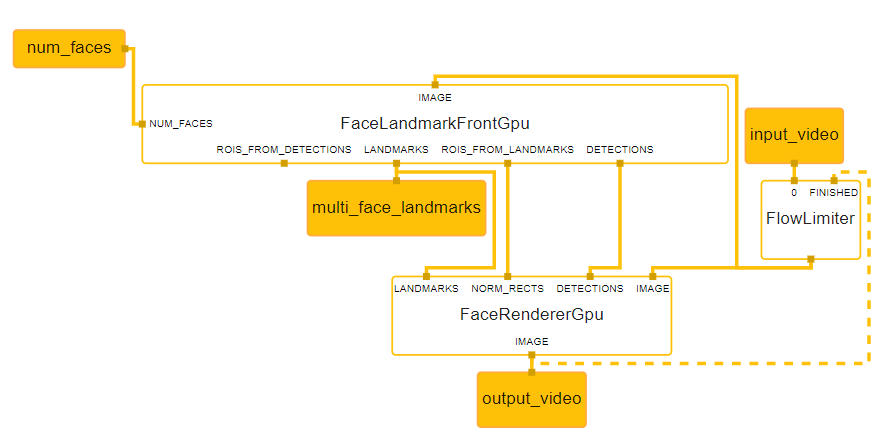
\includegraphics[width=15cm]{imagenes/faceMesh.png}
	\caption{MediaPipe Graph utilizado en FaceMesh}
	\label{fig:faceMesh}
\end{figure}

Por tanto, el procesamiento de una imagen en este modelo sigue dos pasos. El primero (1) toma la imagen de entrada, capturada por la cámara, es procesada por un detector de caras \textit{lightweigth}, llamado \textit{BlazeFace}, y produce unos rectángulos que definen el perímetro donde se encuentra la cara, conjuntamente con un par de puntos de interés superficiales (ojos, boca y nariz). Estos puntos se utilizarán para alinear la cara para el siguiente paso. Y el segundo (2), mediante el rectángulo obtenido en el paso anterior, se recorta la cara de la imagen inicial y es reescalado para utilizarse como entrada de la red neuronal que realiza la prediccion de la malla. (El tamaño de reescalado será entre 256x256 en un modelo completo, hasta 128x128 en el modelo más pequeño). Tras la predicción, se obtiene como salida un vector de coordenadas \textit{landmark 3D}, que serán mapeadas y dibujadas en la imagen original. \cite{faceMesh2}

Las coordenadas que se obtienen como salida estan compuestas por unas coordenadas x e y provenientes de localizaciones del plano 2D propio de la imagen. Mientras que, la coordenada z es interpretada como una profundidad relativa a un centro de masa que compone la malla de la cara.

Se utilizan dos modelos para el funcionamiento de \textit{FaceMesh}. El primero de ellos dedicado a la detección facial, llamado BlazeFace (mencionado anteriormente). Este es un modelo \textit{lightweight} creado para GPU móviles, llegando a una velocidad de procesamiento de entre 200 a 1000 fps en dispositivos móviles punteros. Es inspirado en los modelos \textit{MobileNet}, tanto la primera version como la segunda, provenientes del \textit{framework} SSD (\textit{Single Shot Multibox Detector}). Este modelo produce una salida compuesta por un rectángulo perimetral y 6 puntos de interés faciales. \cite{blazeface}

El segundo modelo, \textit{Face Landmark Model}, es generado mediante \textit{Transfer Learning} buscado una serie de objetivos: crear coordenadas 3D (mencionadas anteriormente) y conseguir mostrarlas en la imagen de salida de forma correcta. \cite{faceMesh} El \textit{Transfer Learning} es una técnica de \textit{Machine Learning} donde se puede hacer uso de un modelo preentrenado para personalizarlo y usarlo en una tarea determinada. Conviene destacar que un modelo entrenado es una red almacenada, entrenada previamente con un conjunto de datos con el objetivo de realizar una tarea de clasificación de imágenes a gran escala. \cite{transferLearning}

\textit{FaceMesh} propone una implementación mediante \textit{TensorFlow Lite} que dispone de dos formatos: CPU y GPU, que presentan un rendimiento en dispositivos moviles (\textit{Pixel3}, \textit{Pixel2} y \textit{iPhoneX}) muy fluido, impresionado sobre todo su funcionamiento sobre CPU. (Figura \ref{fig:faceMeshRen}) \cite{faceMesh3}

\begin{figure}[htp]
	\centering
	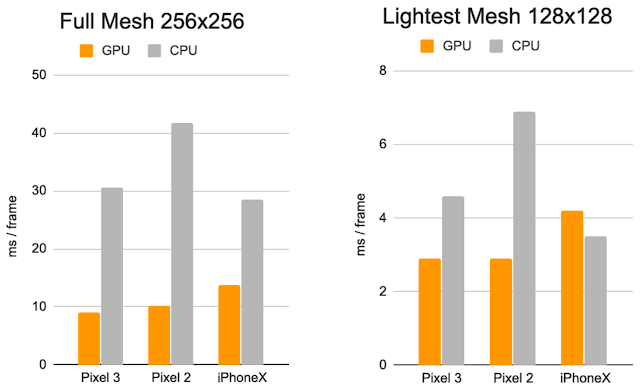
\includegraphics[width=10cm]{imagenes/rendFaceMesh.png}
	\caption{Rendimiento de FaceMesh sobre dispositivos móviles}
	\label{fig:faceMeshRen}
\end{figure}

\subsection*{Prototipo}

Uso de \textit{FaceMesh} del framework \textit{MediaPipe} y un detector basado en \textit{Haar-like features}, como el mencionado en el \textit{paper} de Viola \& Jones (\ref{haar-like}).

% Explicar mi prototipo

\newpage
\section{Tensorflow}

Posible añadido de AlexNet si es útil.

\begin{itemize}
	\item Plantear idea
	\item Procedimiento
	\item Diferentes tipos de modelos
	\item Mostrar funcionamiento y aplicación al objetivo
\end{itemize}

\newpage
\section{Comparación}